\documentclass[10pt,a4paper]{article}
\usepackage[latin1]{inputenc}
\usepackage{amsmath}
\usepackage{amsfonts}
\usepackage{amssymb}
\usepackage{graphicx}
\usepackage{dirtytalk}
\begin{document}
	\section{Beam Energy Corrections}
\begin{enumerate}
	\item
	\say{Clarify if the photon-energy corrections derived and reported in the note were obtained after the application of the phi-dependent momentum corrections reported in 3.3.1. This correction should be derived after e-loss and phi-dependent momentum corrections are applied.}\\
	Stated on page 75 of the note procedures:\\
	''To validate the corrections of the entire g12 data set, the missing neutron mass was recalculated for each run, shown in Fig. 72, using several correction schemes, i.e. a scheme of just ''energy-loss`` corrections, a scheme of ''energy-loss`` and momentum corrections (JTG PCor), a scheme of ''energy-loss``, momentum corrections (JTG PCor) and beam corrections (MK BeamCor) and a scheme of ?energy-loss? and beam corrections (MK BeamCor). It can be seen in Fig. 72 that the only scheme that sufficed was the combination of ''energy-loss`` and beam corrections.``\\ However, the plot was modified, making the above statement not understandable. In Figure~\ref{fig:beam_cor_progession} below shows the plot that this text is referring to. \\
	It should be noted that one method of deriving the momentum corrections before the beam corrections did not improve either the neutron mass measurement or the proton mass measurement. This can be seen in Figure~\ref{fig:beam_cor_progession} by the red data points. Therefore the beam corrections were derived after e-loss but before the phi-dependent momentum corrections. It also should be noted that after the beam corrections were derived and after the phi-dependent momentum corrections were derived, the beam correction algorithm was re-ran to investigate any possible systematic, however the ratio of the largest derivation, for a run, was on the order of $10^{-4}$ which had only a 0.3~MeV increase at 1~GeV photon beam energy.
	 	\begin{figure}[h!]\begin{center}
	 			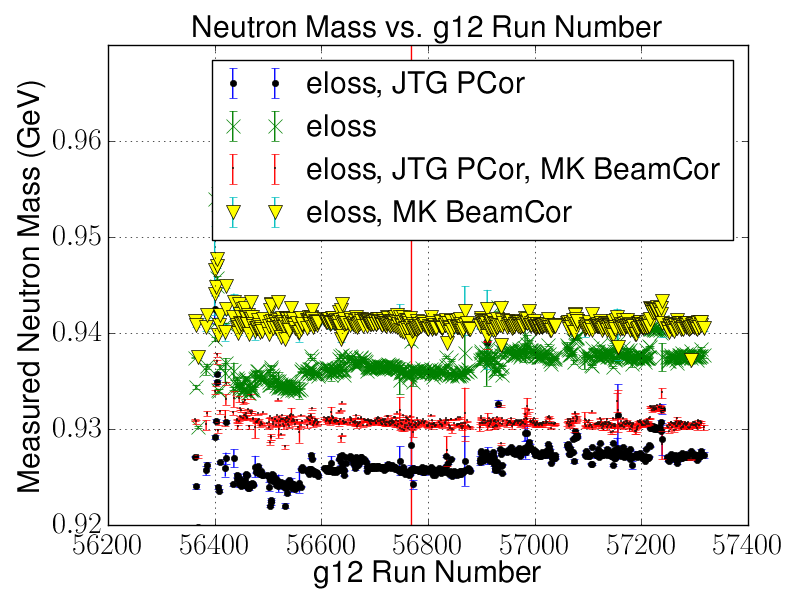
\includegraphics[width=200 pt, height=200 pt]{C3pi_allcorr_neutron_rxr.png}
	 			\caption[Plot showing the series of analyses that contributed to the final chain of procedures for the beam correction]{\label{fig:beam_cor_progession}Plot showing the series of analyses that contributed to the final chain of procedures for the beam correction.}
	 		\end{center}\end{figure}
	 	\end{enumerate}
\end{document}